

In this section the constraints of the superconducting Surface-17 quantum processor developed at QuTech by Di Carlo's group are summarized. To operate on this kind of qubits, analogue signals with a specific frequency, amplitude and envelop are sent.

\subsection{Superconducting quantum processor architecture}
\label{sec:topology}

Figure \ref{fig:sc_17} shows a schematic of the layout for the Surface-17 chip where the circles represent the qubits \cite{versluis2016scalable} and the different colors the frequency used for single-qubit microwave control. In order to perform a single-qubit gate microwave pulses are used, whereas flux-pulses (qubit specific detuning sequence) are used for two-qubit gates. 
To this purpose, every qubit has a dedicated flux-control line (yellow) and microwave-drive line (red) to control the qubit frequency and send operating waves, respectively.
Several qubits are connected through a readout resonator (in purple) to the feedlines (diagonal blue lines) that are used for measuring them. Note that readout resonators are simultaneously interrogated using frequency-division multiplexing.
Finally, only qubits connected by bus resonators (in orange) can interact, this is the nearest-neighbour constraint. 
For more details, please read \cite{versluis2016scalable,versluis2017scalable}.

[ADD LEGEND TO \ref{fig:sc_17}]


Figures \ref{fig:simple_sc_17}  show a schematic of the topology for the Surface-17 quantum chip.
Circles represent the \textbf{qubits}  and the \textbf{edges} represent the 'connections' or possible interactions between them.
Numbers  are the physical addresses of the qubit. As we just mentioned the different colors represent the frequency for single-qubit microwave control: red for $f_1$, blue and green for $f_2$ and pink for $f_3$.


\begin{figure}[h!]
\centerline{\subfigure[Schematic of the realization of SC-17 chip \cite{versluis2016scalable}]{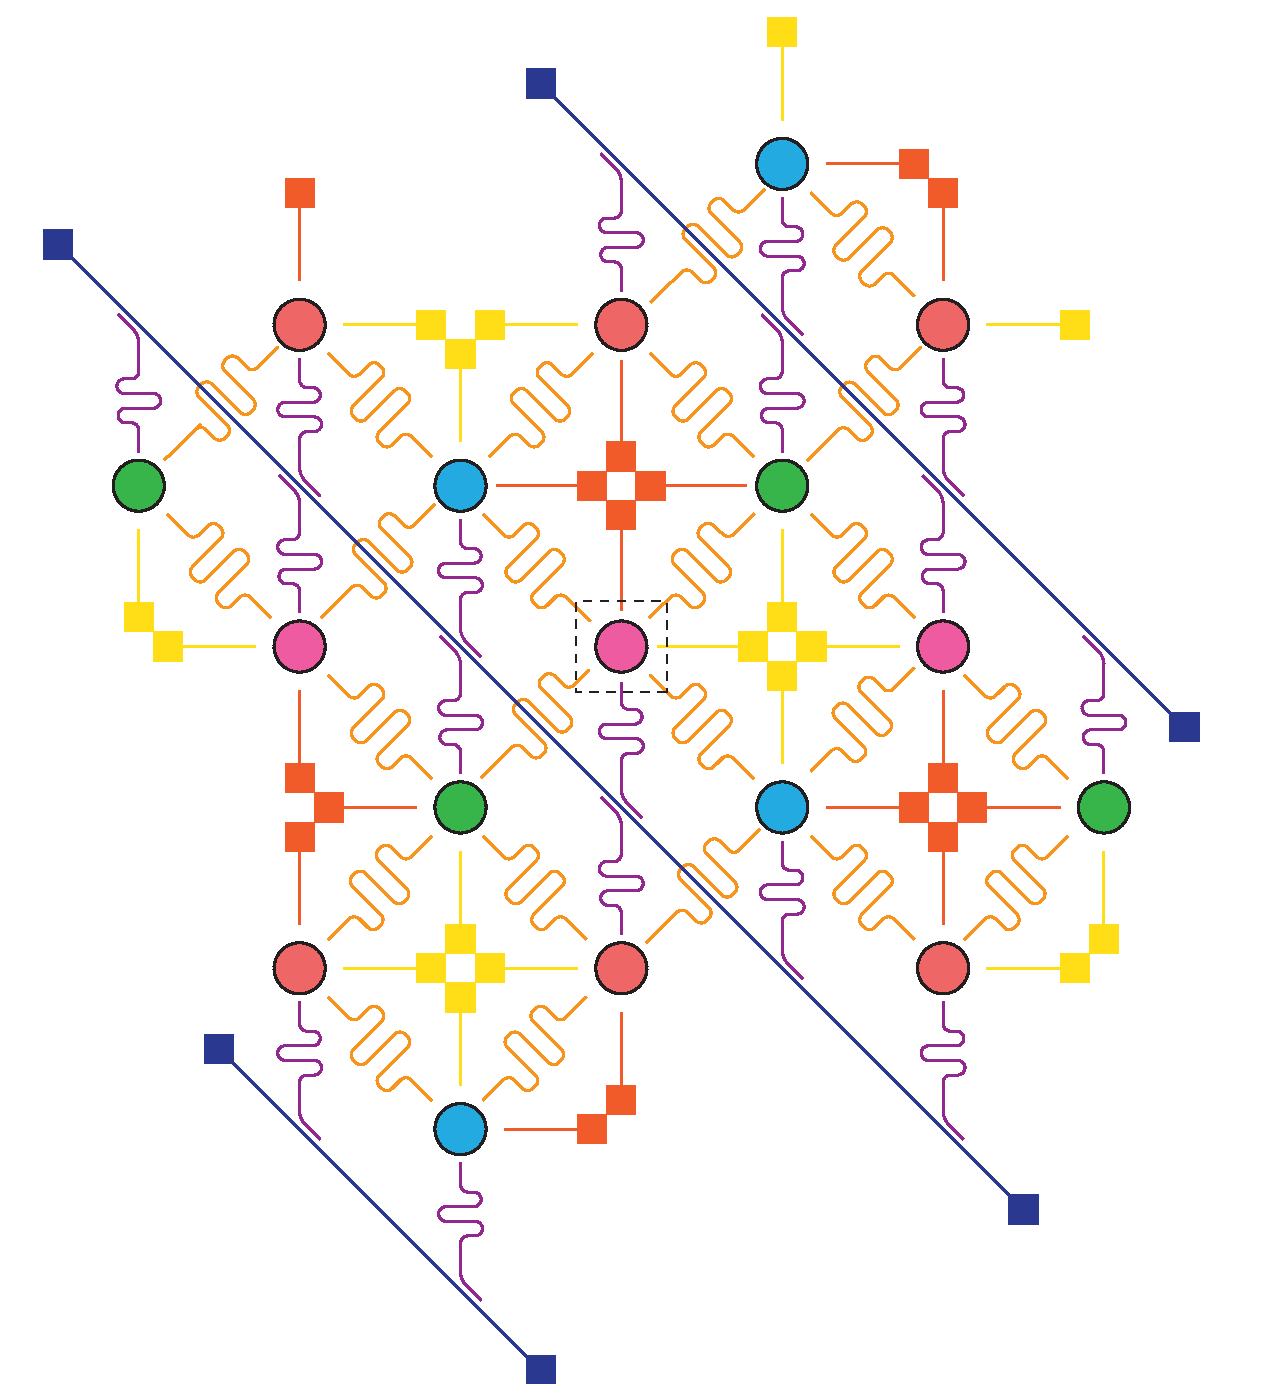
\includegraphics[width=3in]{figures/sc-17}
\label{fig:sc_17}}
\subfigure[Simpler layout of the SC-17. All the examples will refer to this picture]{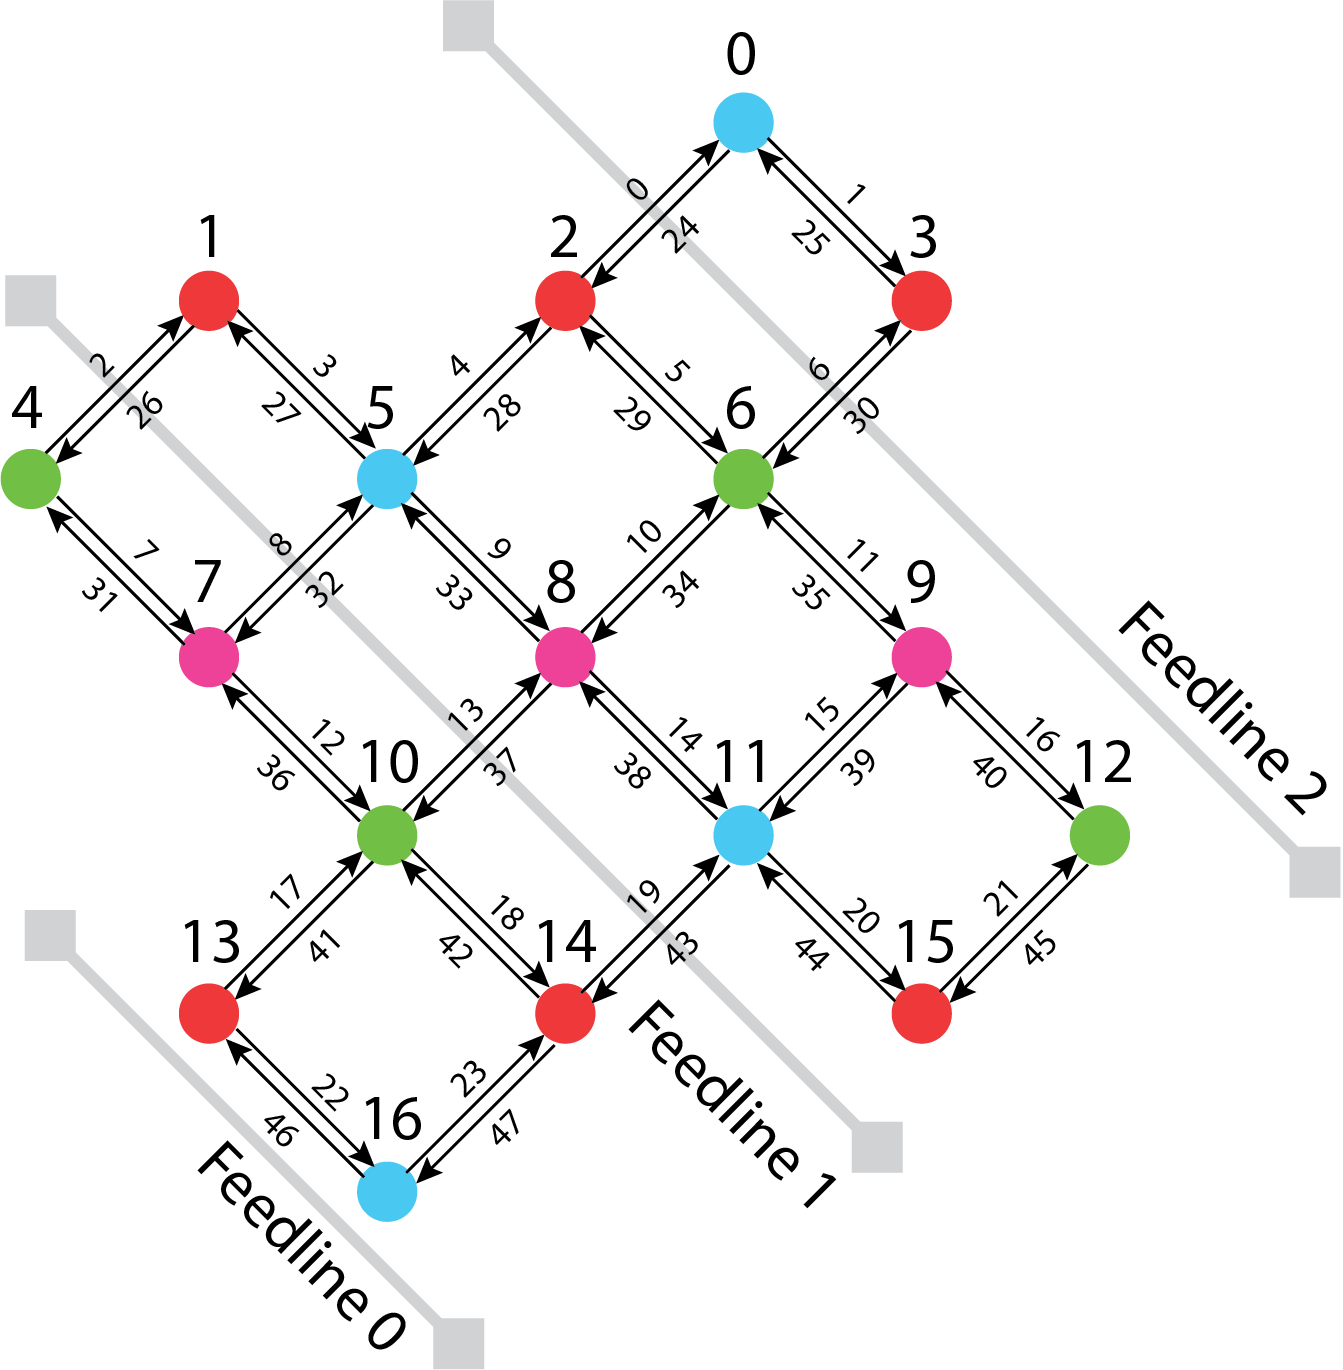
\includegraphics[width=3.5in]{figures/sc17_w_cnnct.png}
\label{fig:simple_sc_17}}}
\caption{SC-17 chip layouts describing its architecture}
\label{Surafce17b}
\end{figure}


%In the SC-7 the connections are characterized as the black lines while in the SC-17 are illustrated as the orange waves.
%As one may predict, this will lead us to one of the main constraints, the \emph{nearest neighbors} restriction.


\newpage

\subsection{Gate set, gate time and gate fidelity}
\label{sec:orgd576c64}

In order to perform universal computation, a whole set of universal gates should be executable in a given device.
However, not all kind of gates are supported in real quantum processors.
In our case, any kind of single qubit rotation can be performed on the superconducting quantum processor, but gates need to be calibrated before performing any experiment and obviously one cannot calibrate infinite amount of gates. Furthermore, Z rotations do not perform very well on this kind of superconducting qubits. Based on these observations, we will limit single qubit gates to X and Y rotations, in which the most common are  $\pm$ 90 (degrees) and $\pm$ 180. Conditional-phase (CZ) gates and measurement in the Z basis are also possible. Therefore, the gates supported (elementary gates) by the superconducting quantum processor are:

\begin{itemize}
\item X gate with arbitrary angle rotation. Most common  \(\pm 90\) and \(\pm180\) degrees rotations
\item Y gate with arbitrary angle rotation. Most common  \(\pm 90\) and \(\pm180\) degrees rotations
%\item Z gate with arbitrary rotations (error rate < 0.1\%)
\item CZ gate 
\item Measurement in the Z basis ($M_{z}$)
\end{itemize}

Table \ref{primitive_gate_time} shows the gate time and the errors rates for single-qubit gates, CZ gate and measurement \cite{versluis2016scalable}. Note that the default basis of measurement will be Z basis unless one specifies.

\begin{table}[h!]
\centering
\caption{The gate time and fidelity of primitive set from experiments. The measurement time includes both measuring and depletion time.}
\label{primitive_gate_time}
\begin{tabular}{lll}
\hline  
\textbf{Gate type}    & \textbf{Gate time} & \textbf{Fidelity}       \\
\hline
Single-qubit & 20 ns     &  $\sim 99.97 \%$ \\
CZ           & 40 ns     & $\sim 99.93 \%$           \\
$M_{z}$  & 600 ns    & $\sim 99.5 \%$     \\  
\hline
\end{tabular}
\end{table}

For the mapping process, we assume that arbitrary rotations and multi-qubit gates are first decomposed to the Clifford+T group, \{H,T,S,CNOT\}. Although this is a universal gate set that is not directly supported by the quantum chip. 
These gates need to be further decomposed into the elementary gates as shown in Figure \ref{fig:decompositions} and their gate time is shown in Table \ref{uni_set_gatetime}.
%\textcolor{red}{We still need to include SWAP decomposition}

\textcolor{red}{Daniel, Table 3.3 is not mentioned in the text.}

  \begin{figure}[t!]     
\begin{center}
%\resizebox{\textwidth}{!}{%

\begin{minipage}{\textwidth}
\Qcircuit @C=1em @R=.7em {
& \gate{Z} & \qw & \push{\equiv} &  & \gate{X} & \gate{Y} & \qw \\
}
\end{minipage}

\vspace{1cm}

\begin{minipage}{\textwidth}
\Qcircuit @C=1em @R=.7em {
    & \gate{H} & \qw & \push{\equiv} & & \gate{Y_{\text{-90}}} & \gate{Z} & \qw & \push{\equiv} & & \gate{Z} & \gate{Y_{\text{+90}}} & \qw & \push{\equiv} & & \gate{X} & \gate{Y_{\text{-90}}} & \qw\\
}
\end{minipage}     

\vspace{1cm}

\begin{minipage}{\textwidth}
\Qcircuit @C=1em @R=.7em {
& \gate{T} & \qw & \push{\equiv} &  & \gate{H} & \gate{X_{+45}} & \gate{H} & \qw & \push{\equiv} &  & \gate{Y_{\text{+90}}} & \gate{X_{+45}} & \gate{Y_{\text{-90}}} & \qw \\
}
\end{minipage}

\vspace{1cm}

\begin{minipage}{\textwidth}
\Qcircuit @C=1em @R=.7em {
& \gate{T^{\dagger}} & \qw & \push{\equiv} &  & \gate{H} & \gate{X_{-45}} & \gate{H} & \qw & \push{\equiv} &  & \gate{Y_{\text{+90}}} & \gate{X_{-45}} & \gate{Y_{\text{-90}}} & \qw \\
}
\end{minipage}

\vspace{1cm}

\begin{minipage}{\textwidth}
\Qcircuit @C=1em @R=.7em {
& \gate{S} & \qw & \push{\equiv} &  & \gate{H} & \gate{X_{+90}} & \gate{H} & \qw & \push{\equiv} &  & \gate{Y_{\text{+90}}} & \gate{X_{+90}} & \gate{Y_{\text{-90}}} & \qw \\
}
\end{minipage}

\vspace{1cm}

\begin{minipage}{\textwidth}
\Qcircuit @C=1em @R=.7em {
& \gate{S^\dagger} & \qw & \push{\equiv} &  & \gate{H} & \gate{X_{+90}} & \gate{H} & \qw & \push{\equiv} &  & \gate{Y_{\text{+90}}} & \gate{X_{-90}} & \gate{Y_{\text{-90}}} & \qw \\
}
\end{minipage}

\vspace{1cm}

%\begin{minipage}{\textwidth}
%\Qcircuit @C=1em @R=.7em {
% & \ctrl{1} & \qw & \push{\equiv} &  & \qw & \ctrl{1} & \qw & \qw & \push{\equiv} &  & \qw & \qw & \ctrl{1} & \qw & \qw & \qw\\
% & \targ & \qw &  &  & \gate{H} & \control \qw & \gate{H} & \qw &  &  & \gate{Y_{\text{-90}}} & \gate{X} & \control \qw & \gate{Y_{\text{-90}}} & \gate{X} & \qw\\
% }
% \end{minipage}

\begin{minipage}{\textwidth}
\Qcircuit @C=1em @R=.7em {
 & \ctrl{1} & \qw & \push{\equiv} &  & \qw & \ctrl{1} & \qw & \qw \\
 & \targ & \qw &  &  & \gate{Y_{-90}} & \control \qw & \gate{Y_{+90}} & \qw\\
 }
 \end{minipage}
 
 \vspace{1cm}
\begin{minipage}{\textwidth}
\Qcircuit @C=1em @R=.7em {
 & \qswap & \qw  & \push{\equiv}& &\ctrl{1} &\targ & \ctrl{1}&\qw &\push{\equiv}& &\qw&\ctrl{1}&\gate{Y_{-90}}&\control \qw&\gate{Y_{+90}}&\ctrl{1}&\qw&\qw\\
 & \qswap \qwx& \qw & & & \targ &\ctrl{-1}& \targ&\qw& & & \gate{Y_{-90}} &\control \qw&\gate{Y_{+90}}&\ctrl{-1}&\gate{Y_{-90}} &\control \qw&\gate{Y_{+90}}& \qw\\
 }
 \end{minipage}
%}

\end{center}

\caption{Decomposition in the X-Y-Z-CZ set of the Clifford + T gates that are not directly supported in the quantum chip}
\label{fig:decompositions}


\end{figure}


\begin{table}[bth!]
\centering
\caption{The gate time for the universal set \{H,S,T,CNOT\}.} 
\label{uni_set_gatetime}
\begin{tabular}{cr}
\hline
Gate type & Gate time \\ \hline
X         & 20 ns     \\ 
Y         & 20 ns     \\ 
Z         & 40 ns     \\ 
H         & 40 ns     \\ 
S/Sdag    & 60 ns          \\ 
T/Tdag    & 60 ns          \\ 
CNOT      & 80 ns     \\ 
SWAP      & 200 ns    \\ 
$M_{Z}$         &  600 ns          \\ \hline
\end{tabular}
\end{table}

\begin{table}[bth!]
\centering
\caption{The gate time for the universal set allowed in the devices $\{R_{X},R_{Y},CZ,M_{Z}\}$}.
\label{sc_set_gatetime}
\begin{tabular}{cr}
\hline
Gate type & Gate time \\ \hline
$R_{X}(\pm 45, \pm90)$         & 20 ns     \\ 
$R_{Y}(\pm 45, \pm90)$       & 20 ns     \\ 
CZ        & 40 ns     \\ 
$M_{Z}$         &  600 ns          \\ \hline
\end{tabular}
\end{table}

%\newpage
In the next sections, the different constraints of the superconducting quantum chip will be explained in detail. Note that we will distinguish two kind of constraints: the ones coming from the quantum chip- e.g. nearest-neighbour interactions- that we call \textbf{hardware constraints} and the ones from the electronics control setup - e.g. qubits operated by the same AWG- called \textbf{electronics constraints}.






\subsection{Qubits interaction constraint}
\label{sec:org77a3a48}

In Surface-17 each qubit is connected to a maximum of four qubits, the nearest-neighbours, limiting the possible interactions -e.g. two-qubit gate- between them (hardware constraint). This constraint will make that qubits that need to interact and are not place in neighboring positions will need to be moved to adjacent positions. Quantum states in superconducting technology can be `moved' by using SWAP operations.


%It is the origin of the mapping problem.
%Therefore, a mapping pass that  is required to run any quantum algorithm in a physical device.




This constraint implies that in Surface-17 (see Figure \ref{fig:simple_sc_17})





% \linebreak[4]
\begin{minipage}[t]{.45\textwidth}

It is possible to do:

\begin{minted}[frame=lines,fontsize=\scriptsize,linenos,breaklines,breakanywhere]{c}
CZ q[1],q[5]
CZ q[8],q[6]
CZ 1Figure\end{minted}

\end{minipage}
\hfill %\hspace{1cm}
\begin{minipage}[t]{.45\textwidth}

but impossible to do (directly, without any mapping):

\begin{minted}[frame=lines,fontsize=\scriptsize,linenos,breaklines,breakanywhere]{c}
CZ q[1],q[2]
CZ q[0],q[16]
\end{minted}

\end{minipage}

The code shown here and in the next sections is written in an eQASM fashion.
The letters represent the kind of gate operation and the number will refer to the qubit number in the Surface-17 layout (Figure \ref{fig:simple_sc_17}).
Also, the character '\texttt{|}' represents the operations that can be executed in parallel. 



% \section{Dependency operation constraint (Hard)}

% \label{sec:org73a281f}

% Qubits can be, exclusively, in one of the following states:

% \begin{itemize}
% \item Idling
% \item Being used in a single- or multi-qubit gate
% \item Being measured
% \end{itemize}

% \begin{minipage}[t]{.45\textwidth}

% Then,

% It is possible to do:

% \begin{minted}[frame=lines,fontsize=\scriptsize,linenos,breaklines,breakanywhere]{c}
% X 1
% Y 1
% \end{minted}

% \end{minipage}
% \hfill %\hspace{1cm}
% \begin{minipage}[t]{.45\textwidth}

% but not:

% \begin{minted}[frame=lines,fontsize=\scriptsize,linenos,breaklines,breakanywhere]{c}
% X 1 | Y 1
% \end{minted}

% \end{minipage}

% This constraint will affect the scheduling of operation, as there is a dependency between gates.

\subsection{Frequency constraint}
\label{sec:orgff4c391}

\subsubsection{Single-qubit gates}

In order to perform single-qubit gates, electromagnetic microwaves are sent. As shown in Figures \ref{fig:simple_sc_17}, three or four different frequencies for single-qubit microwave control can be used in Surface-17. In principle, any qubit can be operated individually and then any combination of single-qubit gates can be performed in parallel. However, qubits using the same frequency are controlled by the same Quantum Waveform Generator (QWG) and then they are limiting the possible parallelism of operations.


\begin{table}[h!]

\caption{\label{T4}
Frequency groups for Surface-17 when using 3 different frequencies.}
\centering
\begin{tabular}{lll}
 & \\
\hline
QWG & Qubits & Frequency Group\\
\hline
\cellcolor{red!25}  0 & \cellcolor{red!25} 1, 2, 3, 13, 14, 15 & \cellcolor{red!25} $f_1$\\
\cellcolor{pink!25}  1 & \cellcolor{pink!25} 7, 8, 9 & \cellcolor{pink!25} $f_3$\\
\cellcolor{Aquamarine!25}  2 & \cellcolor{Aquamarine!25} 0, 4, 5, 6, 10, 11, 12 16 & \cellcolor{Aquamarine!25} $f_2$\\
\hline
\end{tabular}
\end{table}
%\end{minipage}

\newpage
It is not possible to perform two different single-qubit gates at the same time on qubits using the same frequency and operated by the  same QWG. For instance in SC-17,

\begin{minipage}[t]{.45\textwidth}

It is possible to do:

\begin{minted}[frame=lines,fontsize=\scriptsize,linenos,breaklines,breakanywhere]{c}
{ X q[1] | X q[7] }
8{ X q[6] | Y q[7] }
{ X q[1] | X q[2] | X q[5] | X q[0] }
{ Y q[10] | Y q[4] }

\end{minted}

\end{minipage}
\hfill %\hspace{1cm}
\begin{minipage}[t]{.45\textwidth}

But not

\begin{minted}[frame=lines,fontsize=\scriptsize,linenos,breaklines,breakanywhere]{c}
{ X q[1] | Y q[2] }
{ X q[5] | Y q[0] }
{ X q[10] | Y q[4] }
{ X q[7] | Y q[9] }
\end{minted}

\end{minipage}

Obviously, it is not possible to perform more than one single-qubit gate on the same qubit at the same time (gate dependency).

\subsubsection{Two-qubit gates}

In order to perform a two-quibt gate in superconducting qubits, interacting qubits need to be brought to a specific close frequencies \cite{versluis2016scalable}. More specifically, $CZ_f$ gates are performed between qubits at $f^{int}_1$ and $f_2$ or at $f^{int}_2$ and $f_3$ as shown in Figure \ref{detuning}. In addition, the qubits that share a connection with the qubits performing a 2-qubit gate need to be detunned away. This limits the amount of two-qubit gates that can be performed in parallel (hardware constraint). %In addition, note that, different frequency arrangements can be used as shown in Figure \ref{sequence}. 


\begin{figure}[h!]
  \centerline{
    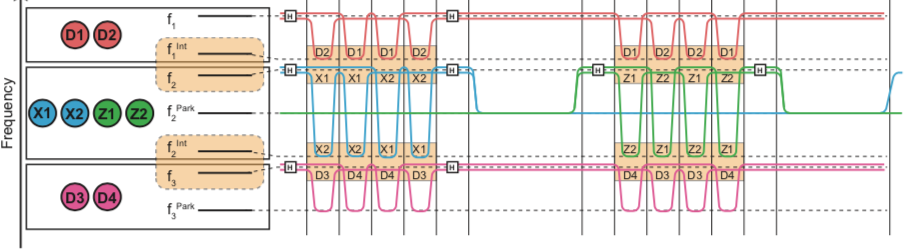
\includegraphics[width=5in]{figures/detuning.png}
    }
\caption{Frequency arrangement and detuning frequencies for the qubits in the unit cell.}
\label{sequence}
\end{figure}


Based on the notation in Figure \ref{cell} and assuming the frequency scheme of Figure \ref{detuning} we can formulate the following: 1) If a two-qubit gate is being performed between D1 (D2) and X1 (X1 or Z1), D2 (D1) cannot interact with X1 or Z1 (X1) at the same time; 2) In the same way, if a two-qubit gate is being performed between D3 (D4) and X1 or Z2 (X1 or Z1 or X2 or Z2), D4 (D3) cannot interact with X1 or Z1 or X2 or Z2 (X1 or Z2) at the same time. Obviously,  if a two-qubit gate is being performed between two qubits, the qubits involved can not perform another single- or two-qubit gate at the same time.
%As an example, a summary of the gates that cannot be performed in paralallel in SC-7 is shown in Table \ref{parallelCZ}.

%% \begin{table}[h!]
%% \centering
%% \caption{Allowed and not allowed parallel CZ gates in the unit cell.}
%% \label{parallelCZ}
%% \small
%% \resizebox{0.80\textwidth}{!}{
%% \begin{tabular}{|c|c|c|}
%% \hline
%% CZ gate    & NOT Possible two-qubit gates in parallel                  & NOT Possible single-qubit gates   \\ \hline
%% D1-X1      & D2-X1, D3-X1, D4-X1, D2-Z1                      &  X2, D1, X1\\ \hline
%% D2-X1      & D1-X1, D3-X1, D4-X1, D2-Z1                      &  X2, D2, X1 \\ \hline
%% D3-X1      & D1-X1, D2-X1, D4-X1, D3-Z2, D4-Z1, D4-Z2, D4-X2 &  D4, D3, X1                     \\ \hline
%% D3-Z2      & D3-X1, D4-X1, D4-X2, D4-Z1, D4-Z2               &  D4, D3, Z2       \\ \hline
%% D4-X1      & D1-X1, D2-X1, D3-X1, D4-Z1, D4-Z2, D4-X2, D3-Z2 &  D3, D4, X1                     \\ \hline
%% D2-Z1             & D2-X1, D4-Z1, D1-X1                      &  Z2, D2, Z1 \\ \hline
%% D4-Z2      & D3-X1, D3-Z2, D4-X1, D4-X2, D4-Z1               &  D3, D4, Z2        \\ \hline
%% D4-Z1      & D3-X1, D3-Z2, D4-X1, D4-X2, D4-Z2, D2-Z1        &  D3, D4, Z1               \\ \hline
%% D4-X2      & D3-X1, D3-Z2, D4-X1, D4-Z1, D4-Z2               &  D3, D4, X2       \\ \hline

%% \end{tabular}}
%% \end{table}


%% This can be extended to SC-17 based on the same frequency scheme and the simplified layout shown in Figure \ref{fig:simple_sc_17}.% \textcolor{red}{We need to derive what operations can be performed in parallel and fill Table \ref{parallelCZSC17} in.}

%% %\textcolor{red}{We also need to derive what operations can be performed in parallel for SC-7.}

%% \begin{table}[h!]
%% \caption{Allowed and not allowed parallel CZ gates in SC-17.}
%% \label{parallelCZSC17}
%% \centering
%% \scriptsize
%% \resizebox{0.80\textwidth}{!}{
%% \begin{tabular}{|c|c|c|}
%% \hline
%% CZ gate & Not possible parallel two-qubit gates & Not allowed qubits for single-qubit gates\\
%% \hline
%% Q0-Q2 & Q1-Q5,Q2-Q5,Q2-Q6,Q3-Q0,Q3-Q6 & Q0,Q2,Q5,Q6\\
%% \hline
%% Q0-Q3 & Q0-Q2,Q2-Q6,Q3-Q6,Q2-Q5  & Q0,Q3,Q6\\
%% \hline
%% Q1-Q4 & Q1-Q5,Q2-Q5,Q4-Q7 & Q1,Q4,Q5\\
%% \hline
%% Q1-Q5 & Q1-Q4,Q5-Q7,Q2-Q5,Q5-Q8,Q2-Q0,Q2-Q6 & Q1,Q5,Q4\\
%% \hline
%% Q2-Q5 & Q1-Q4,Q1-Q5,Q2-Q0,Q2-Q6,Q0-Q3,Q3-Q6,Q5-Q7,Q5-Q8 & Q2,Q5,Q0,Q6\\
%% \hline
%% Q2-Q6 & Q1-Q5,Q2-Q5,Q2-Q0,Q6-Q8,Q0-Q3,Q6-Q9,Q3-Q6 & Q2,Q6,Q5,Q0\\
%% \hline
%% Q3-Q6 & Q2-Q5,Q2-Q0,Q2-Q6,Q6-Q8,Q0-Q3,Q6-Q9 & Q3,Q6,Q0\\
%% \hline
%% Q4-Q7 & Q1-Q4,Q5-Q7,Q7-Q10,Q5-Q8,Q8-Q10 & Q4,Q7,Q8\\
%% \hline
%% Q5-Q7 & Q4-Q7,Q1-Q5,Q7-Q10,Q2-Q5,Q5-Q8,Q8-Q10,Q6-Q8,Q8-Q11 & Q5,Q7,Q8\\
%% \hline
%% Q5-Q8 & Q4-Q7,Q1-Q5,Q5-Q7,Q7-Q10,Q8-Q10,Q8-Q6,Q8-Q11,Q6-Q9,Q9-Q11 & Q5,Q8,Q7,Q9\\
%% \hline
%% Q6-Q8 & Q5-Q7,Q7-Q10,Q5-Q8,Q8-Q10,Q2-Q6,Q8-Q11,Q3-Q6,Q6-Q9,Q9-Q11 & Q6,Q8,Q7,Q9\\
%% \hline
%% Q6-Q9 & Q5-Q8,Q8-Q10,Q2-Q6,Q6-Q8,Q8-Q11,Q3-Q6,Q9-Q11,Q9-Q12 & Q6,Q9,Q8\\
%% \hline
%% Q7-Q10 & Q4-Q7,Q5-Q7,Q10-Q13,Q5-Q8,Q8-Q10,Q10-Q14,Q6-Q8 ,Q8-Q11  & Q7,Q10,Q8\\
%% \hline
%% Q8-Q10 & Q5-Q7,Q7-Q10,Q10-Q13,Q5-Q8,Q10-Q14,Q6-Q8,Q8-Q11,Q6-Q9,Q9-Q11 & Q8,Q10,Q7,Q9\\
%% \hline
%% Q8-Q11 & Q5-Q7,Q7-Q10,Q5-Q8,Q8-Q10,Q6-Q8,Q11-Q14,Q6-Q9,Q9-Q11,Q11-Q15,Q9-Q12  & Q8,Q11,Q7,Q9\\
%% \hline
%% Q9-Q11 & Q5-Q8,Q8-Q10,Q6-Q8,Q8-Q11,Q11-Q14,Q6-Q9,Q11-Q15,Q9-Q12 & Q9,Q11,Q8\\
%% \hline
%% Q9-Q12 & Q6-Q8,Q8-Q11,Q6-Q9,Q9-Q11,Q12-Q15 & Q9,Q12,Q8\\
%% \hline
%% Q10-Q13 & Q7-Q10,Q13-Q16,Q8-Q10,Q10-Q14,Q14-Q10,Q11-Q14 & Q10,Q13,Q16\\
%% \hline
%% Q10-Q14 & Q7-Q10,Q10-Q13,Q13-Q16,Q8-Q10,Q14-Q16,Q11-Q14,Q11-Q15 & Q10,Q14,Q16,Q11\\
%% \hline
%% Q11-Q14 & Q10-Q13,Q13-Q16,Q10-Q14,Q14-Q16,Q8-Q11,Q9-Q11,Q11-Q15,Q12-Q15 & Q11,Q14,Q10,Q16\\
%% \hline
%% Q11-Q15 & Q10-Q14,Q14-Q16,Q8-Q11,Q11-Q14,Q9-Q11,Q12-Q15 & Q11,Q15,Q12\\
%% \hline
%% Q12-Q15 & Q11-Q14,Q11-Q15,Q9-Q12 & Q12,Q15,Q11\\
%% \hline
%% Q13-Q16 & Q10-Q13,Q10-Q14,Q14-Q16,Q11-Q14  & Q13,Q16,Q10\\
%% \hline
%% Q14-Q16 & Q10-Q13,Q13-Q16,Q10-Q14,Q11-Q14,Q11-Q15 & Q14,Q16,Q10,Q11\\
%% \hline
%% \end{tabular}
%% }
%% \end{table}

%% \subsubsection*{Summary for single-qubit and two-qubit gates}

%\textbf{Single-qubit gates:} for performing a single-qubit gate on a qubit, one needs to send the required electromagnetic microwave to it.  \textbf{The same} single-qubit gate can be performed in parallel in all or some of the qubits connected to the same QWG. However, it is not possible to perform in parallel a different single qubit-gate in qubits connected to the same QWG.

%\textbf{Two-qubit gates:} in order to perform a two-qubit gate in transmons, interacting qubits need to be brought to a specific close frequencies. In addition, the qubits that share a connection with the qubits performing a 2-qubit gate need to be detunned away. %% For instance, in SC-17, when performing a CZ(11,14), q16 and q10 need to be detunned to $f_{2}^{park}$. Note that it is not possible to perform a single-qubit gate (in parallel with the two-qubit gate) on the qubits that have been detunned to  $f_{1}^{int}$,  $f_{2}^{park}$, $f_{2}^{int}$ or $f_{3}^{park}$.

As an example, in Figure \ref{fig:two_qubit_gate_ex}, a CZ gate is applied between qubits 11 and 14 (\texttt{cz (q[11], q[14])}). Thus, both qubits need to be tuned to closer frequencies -- $f_1^{int}$ and $f_2$ in this case. And, as explained before, in order to not create intereferences between qubits some of them should be detunned away. Specifically, qubits 10 and 16 need to be detunned to $f_2^{park}$ because they share a connection with the qubits performing the CZ gate. This means that no single-qubit gate can be applied to these qubits that are outside their main frequency ($f_2$). And, also, that they cannot perform another two-qubit gate at the same time with any other qubit from the QWG 0 -- the red qubits with main frequency $f_1$ -- because it is required to tune them to $f_2$.

Finally, all the qubits that are already in use cannot be used at the same time. Therefore, qubits 11 and 14 in the example cannot be used in any single- or two-qubit gates.

\textcolor{red}{Delete SC-7 in Figure 3.4}

\begin{figure}[h!]
\centering
%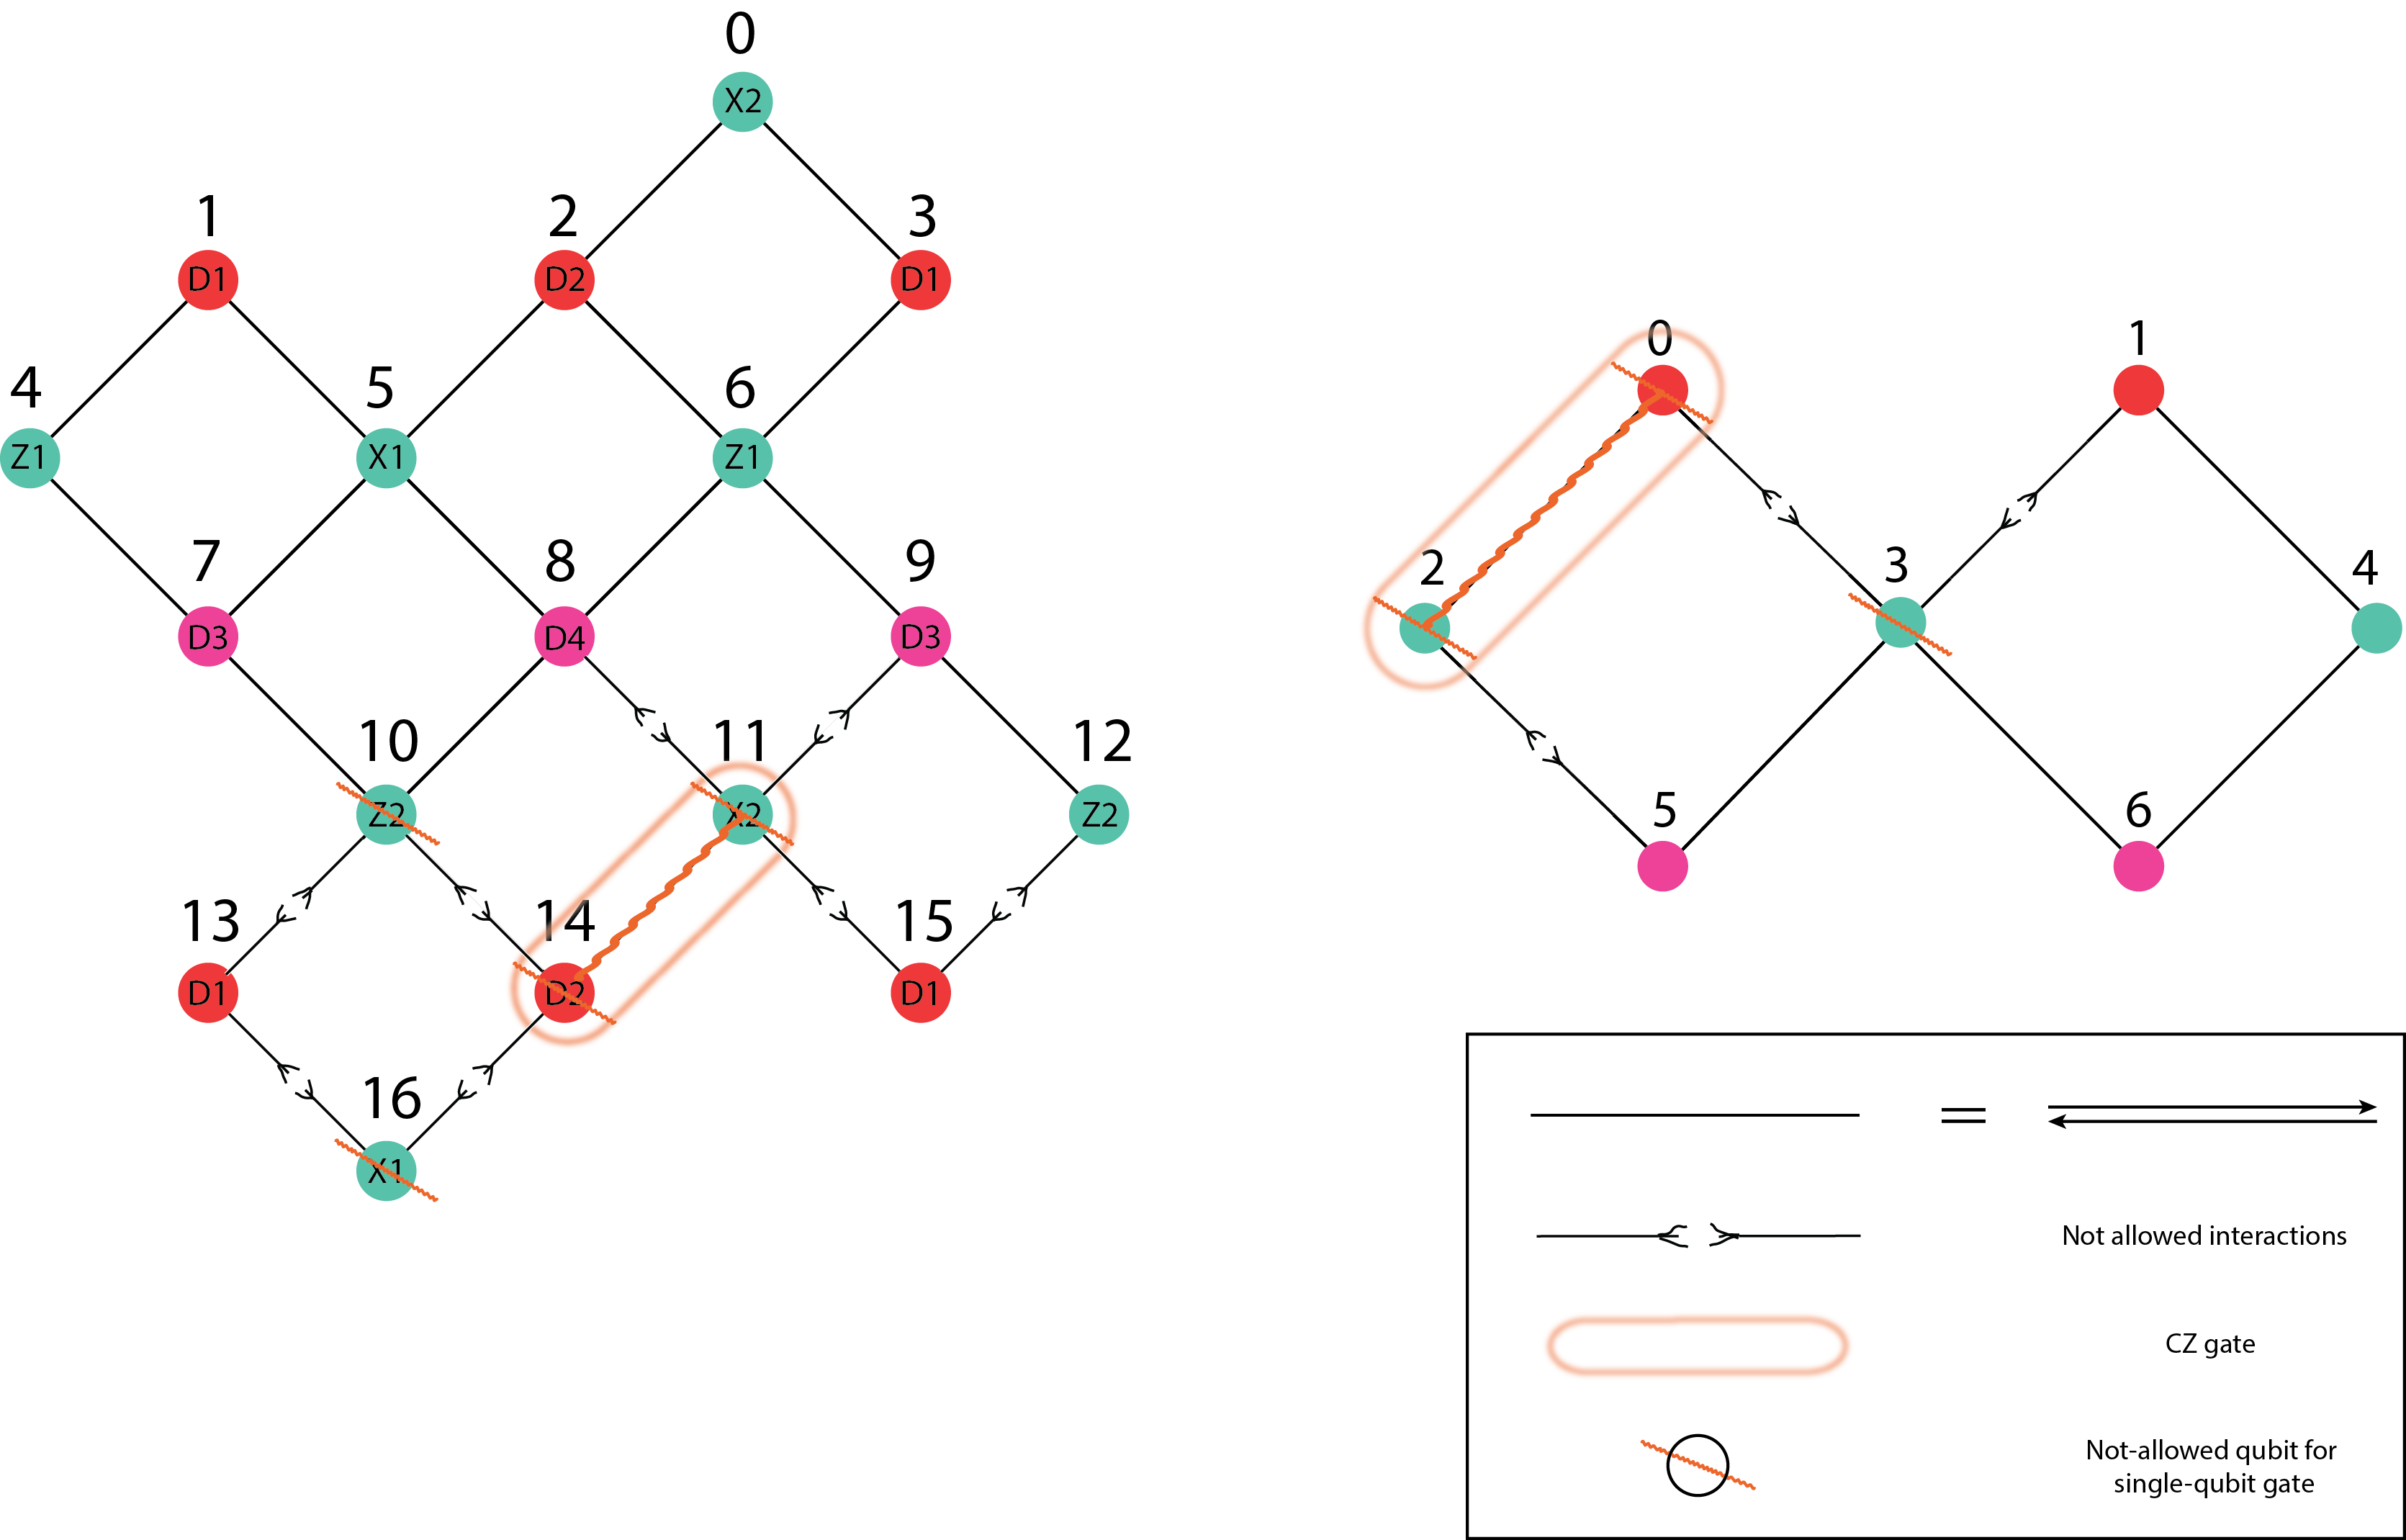
\includegraphics[width=\textwidth]{figures/two_qubit_constraint_sc17.png}
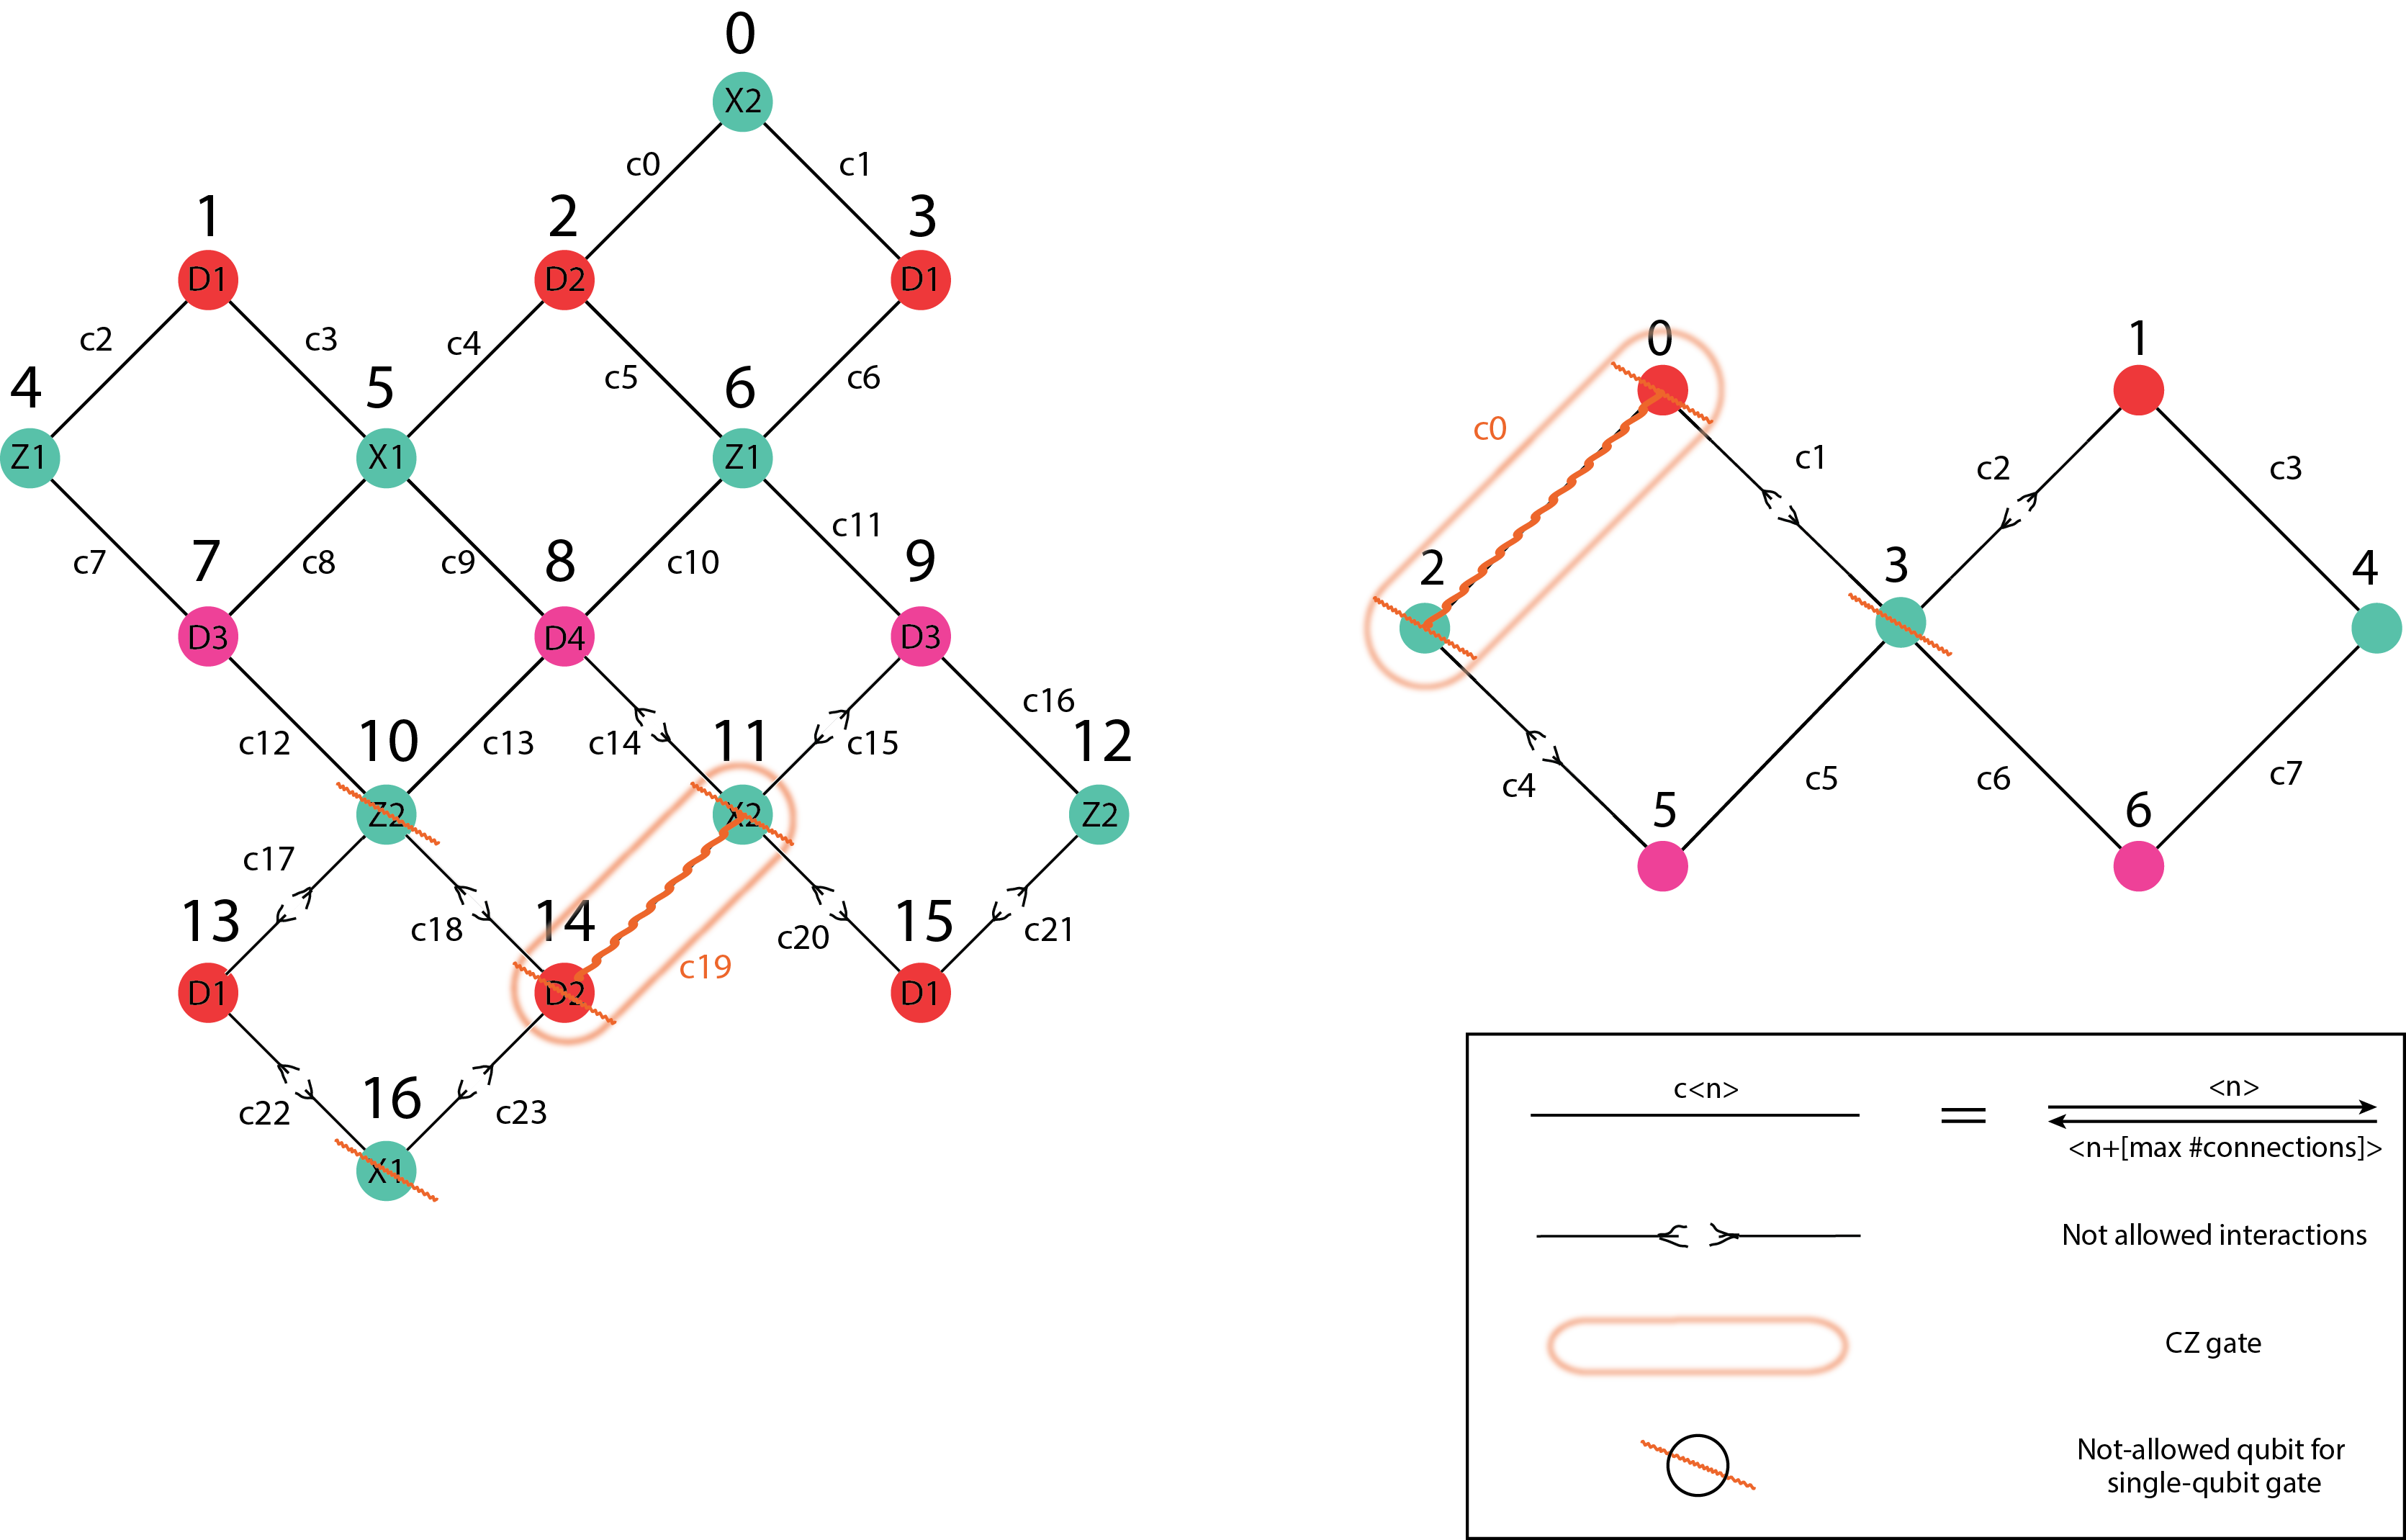
\includegraphics[width=\textwidth]{figures/two_qubit_constraint_sc17_w_cnnct.png}
\caption{\label{fig:two_qubit_gate_ex}
Example of a two qubit gate and allowed and not allowed parallel gates in SC-17}
\end{figure}

%More specifically, the two next connection in the same axis will be forbidden for two-qubit interactions. The first connection as a consequence of the qubit exclusivity constraint because one of the qubits is being used.
%And the second one is a consequence of this constraint.

%In fig. \ref{fig:mesh} a picture of an infinite qubits mesh is drawn.
%In the example, a two-qubit gate is happening between qubits d and e.
%As a consequence, you can see the closer connections that are forbidden and in green the ones that could be use at the same time.

% \begin{figure}[b!]
     
%      \tikzset{cross/.style={cross out, draw=black, fill=none, minimum size=2*(#1-\pgflinewidth), inner sep=0pt, outer sep=0pt}, cross/.default={5pt}}
     
%      \begin{center}
%      \resizebox{\textwidth}{!}{%

% \begin{tikzpicture}[x=5mm,y=5mm]

% \node [circle,fill=black,minimum size=10pt] at (0,0) {};
% \node [circle,fill=black,minimum size=10pt] at (10,0) {};
% \node [circle,fill=black,minimum size=10pt] at (20,0) {};
% \node [circle,fill=black,minimum size=10pt] at (5,5) {};
% \node [circle,fill=black,minimum size=10pt] at (5,-5) {};
 % \node [circle,fill=black,minimum size=10pt] at (15,5) {};
% \node [circle,fill=black,minimum size=10pt] at (25,5) {};
% \node [circle,fill=black,minimum size=10pt] at (15,-5) {};
% \node [circle,fill=black,minimum size=10pt] at (25,-5) {};
% \node [circle,fill=black,minimum size=10pt] at (30,0) {};

% \node [purple] at (1,0) {\huge a};
% \node [purple] at (11,0) {\huge d};
% \node [purple] at (21,0) {\huge g};
% \node [purple] at (6,5) {\huge b};
% \node [purple] at (16,5) {\huge e};
% \node [purple] at (26,5) {\huge h};
% \node [purple] at (6,-5) {\huge c};
% \node [purple] at (16,-5) {\huge f};
% \node [purple] at (26,-5) {\huge i};
% \node [purple] at (31,0) {\huge j};


% \draw (0,0) -- (5,5) node [midway, above, sloped] {};
% \draw (2.5,2.5) node[cross=5pt,rotate=45,red] {};

% \draw (5,5) -- (10,0)  node [midway, above, sloped] {};
% \draw (7.5,2.5) node[cross=5pt,rotate=45,red] {};

% \draw [line width=0.5mm,cyan] (10,0)  -- (15,5) node [midway, above, sloped] {};

% \draw (15,5) -- (20,0) node [midway, above, sloped] {};
% \draw (17.5,2.5) node[cross,rotate=45,red] {};

% \draw (20,0) -- (25,5) node [midway, above, sloped] {};
% \draw (22.5,2.5) node[cross,rotate=45,red] {};

% \draw [green] (20,0) -- (15, -5) node [midway, above, sloped] {};

% \draw (15, -5) -- (10, 0) node [midway, above, sloped] {};
% \draw (12.5,-2.5) node[cross,rotate=45,red] {};

% \draw (10, 0) -- (5, -5) node [midway, above, sloped] {};
% \draw (7.5,-2.5) node[cross,rotate=45,red] {};

% \draw [green] (5, -5) -- (0,0) node [midway, above, sloped] {};

% \draw [green] (20, 0) -- (25,-5) node [midway, above, sloped] {};
% %\draw (22.5,-2.5) node[cross,rotate=45,red] {};

% \draw [green] (25,5) -- (30,0) node [midway, above, sloped] {};


% \draw [green] (30,0) -- (25,-5) node [midway, above, sloped] {};
% %\draw (27.5,-2.5) node[cross,rotate=45,red] {};

% \draw[dotted] (0,0) -- (-5,5);
% \draw[dotted] (0,0) -- (-5,-5);
% \draw[dotted] (30,0) -- (35,5);
% \draw[dotted] (30,0) -- (35,-5);

% \end{tikzpicture}

%      }
%      \end{center}

%           \caption{Example of the connection constraint in an infinite qubits mesh}
%      \label{fig:mesh}


     
%      \end{figure}



\subsection{Measurement constraint}
\label{sec:org58adcb1}

Measuring the qubits is done by using feedlines coupled to several qubits.
For example, in the SC-17 chip, the feedline 1 is used to measure qubits 1, 4, 5, 7, 8, 10, 11, 14 and 15. This will lead us to the last limitation, the \emph{measurement constraint} (hardware constraint). In this case, the measurement on a qubit cannot start when
another qubit coupled to the same feedline is being measured, but it
allows to start measurement on any combination of qubits coupled to
the same feedline at the same time.  Furthermore, there is no dependency between
measurements of any two qubits coupled to different feedlines.



\begin{minipage}[t]{.45\textwidth}

In SC-17, it is possible to do

\begin{minted}[frame=lines,fontsize=\scriptsize,linenos,breaklines,breakanywhere]{c}
  
measure q[0] | measure q[2] | measure q[3] | measure q[6] | measure q[9] | measure q[12]
measure q[1] | measure q[13]
qwait 30
measure q[3] | measure q[8]

\end{minted}

notice that the measurement of qubits 13 and 16 is executed at the same cycle.     

\end{minipage}
\hfill %\hspace{1cm}
\begin{minipage}[t]{.45\textwidth}

On the other hand it is not possible to do

\begin{minted}[frame=lines,fontsize=\scriptsize,linenos,breaklines,breakanywhere]{c}
  
  measure q[2]
  measure q[6]
  
\end{minted}

Note that, in order to measure qubit 2 and 6 in different times, the latter instruction should wait 30 cycles for the first one to finish. In other words, this code is missing a \texttt{qwait 30} instruction.

\end{minipage}
